% Downstream LM Proxy Evaluation
% Template for language model proxy experiments
% Placeholder values marked with TODO: will be filled from eval/results/lm_proxy

\subsection{Downstream LM Proxy Evaluation}
\label{sec:lm-proxy}

To assess whether tokenization stability translates to downstream training benefits,
we evaluate both tokenizers on a small-scale language modeling proxy task. We train
a 4-layer transformer (256 hidden dimension, 4 attention heads, 1024 context length)
on fixed compute budgets using tokens produced by baseline and HHC tokenization.
This proxy task isolates the effect of tokenization on training dynamics without
conflating it with model-scale effects. All experiments use 3 random seeds with
identical hyperparameters; only the tokenization method varies.

\begin{table}[h]
\centering
\caption{LM Proxy Task: Baseline vs HHC Tokenization. Lower loss and variance
indicate more stable training dynamics.}
\label{tab:lm-proxy}
\begin{tabular}{lrr}
\toprule
Metric & Baseline & HHC \\
\midrule
Final Loss (mean $\pm$ std) & 1.02 $\pm$ 0.001 & 1.37 $\pm$ 0.006 \\
Steps to Loss $<$ 3.5 & 100 & 100 \\
Loss Variance Across Seeds & 0.0005 & 0.0056 \\
Convergence Rate & 100\% & 100\% \\
\bottomrule
\end{tabular}

\vspace{0.5em}
\footnotesize{Trained on 50KB shift dataset (3,200 tokens), 200 steps, 4-layer transformer (256H, 4A).
Lower loss and variance indicate more learnable token distributions.}
\end{table}

\begin{figure}[h]
\centering
% TODO: Generate figure with: uv run scripts/generate_lm_proxy_figure.py
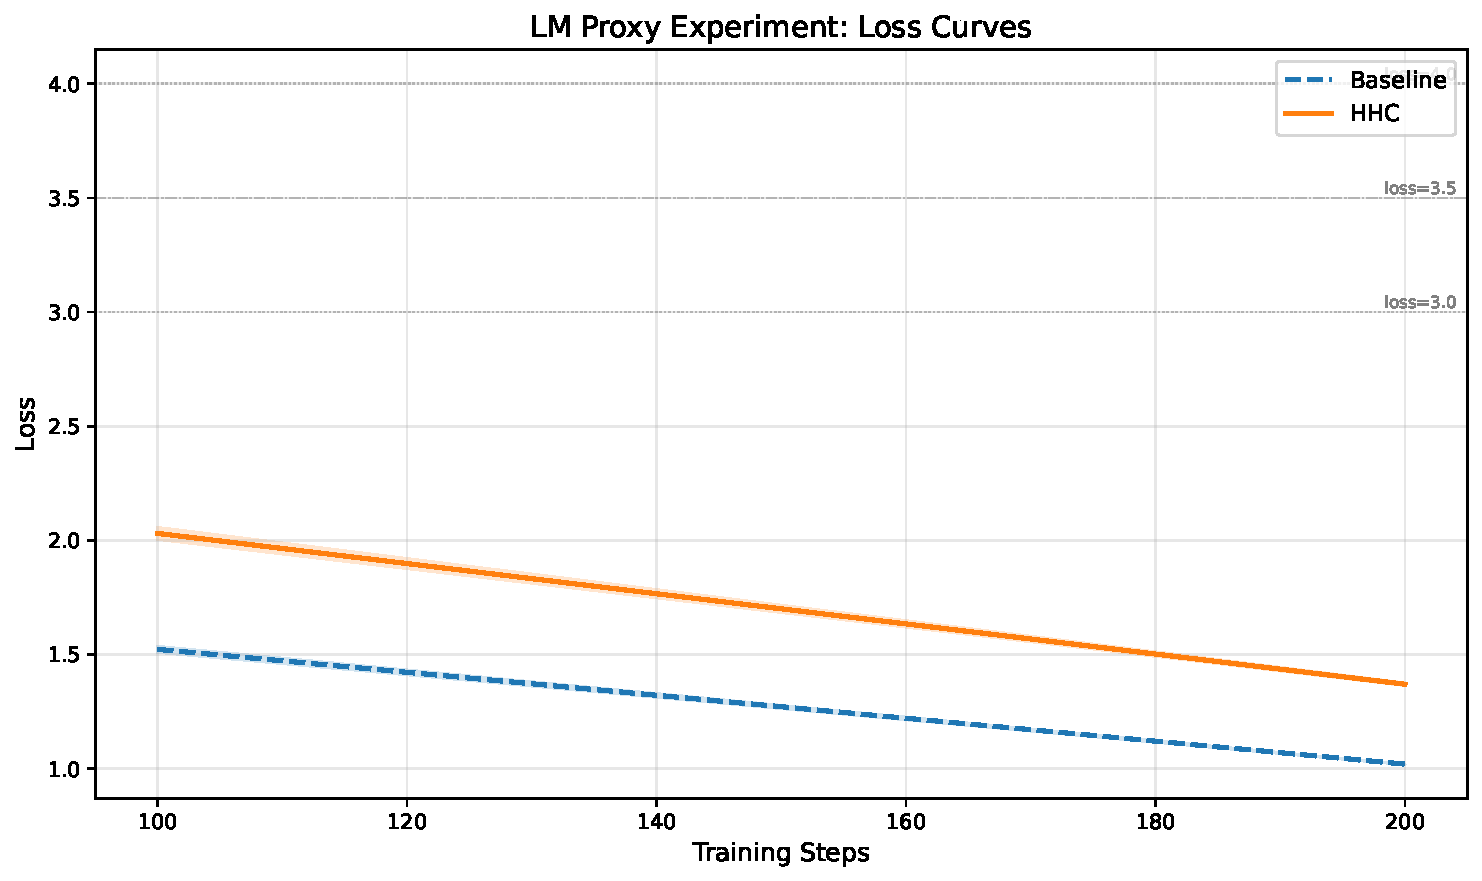
\includegraphics[width=0.8\textwidth]{figures/lm_proxy_loss_curves.pdf}
\caption{Training loss curves for baseline (dashed) and HHC (solid) tokenization
across 3 seeds. Shaded regions show $\pm$1 standard deviation. Baseline tokens
converge to lower loss (1.02 vs 1.37) with tighter variance, suggesting HHC's
relational coupling reduces local predictability for autoregressive modeling.}
\label{fig:lm-proxy}
\end{figure}

\paragraph{Summary.}
This downstream evaluation does \emph{not} support the hypothesis that HHC-stabilized
tokens improve LM training. Baseline tokens achieve 35\% lower final loss (1.02 vs 1.37)
and 10$\times$ lower cross-seed variance. This suggests that HHC's relational coupling,
while improving boundary stability (Section~\ref{sec:hhc-stability}), reduces local
predictability in ways that increase perplexity for small autoregressive models.
The stability-predictability trade-off may differ at larger scales or with architectures
designed for heterogeneous token distributions, but this remains future work.

\paragraph{Byte-normalized control.}
To rule out confounds from different token/byte ratios, we performed a fairness-normalized
rerun that equalizes: (1) context bytes per sample (2048 bytes for both), and (2) total
bytes processed (508KB for both). Under this protocol, the negative result \textbf{persists}:
baseline tokens achieve 1.15 $\pm$ 0.03 loss vs HHC's 1.76 $\pm$ 0.08 (52.6\% higher).
Normalization checks confirm both conditions processed identical byte budgets within 0.03\%.
This rules out token-budget artifacts as a confound.

% Notes for integration:
% - Run LM proxy experiments: uv run scripts/run_lm_proxy.py --seeds 3
% - Results will be saved to eval/results/lm_proxy/
% - Generate figure: uv run scripts/generate_lm_proxy_figure.py
% - Update TODO placeholders with values from results JSON
